\section{Server Architecture}


The following is an overview about how \emph{Studybot} has been created.
Instead of covering all details, the focus here is to communicate the underlying concepts,
which are not unique to this specific chatbot and thereby enable others to apply these patterns in their own development.
\\

\begin{figure}[h]
  \centering
  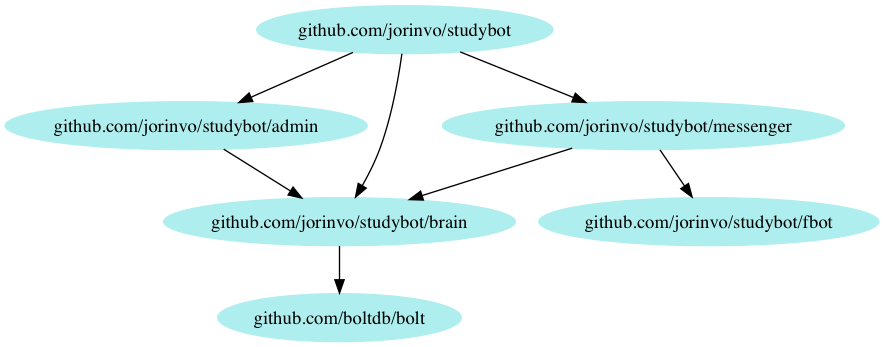
\includegraphics[width=0.8\textwidth]{images/internal-deps.png}
  \caption{Package dependency graph\protect\footnotemark}
	\label{fig:internal-deps}
\end{figure}
\footnotetext{The graph has been created with \emph{godepgraph}~\cite{godepgraph}}

There are numerous resources available today that demonstrate the development of chatbots.
However a majority of existing materials rely on specific services, frameworks or libraries for the implementation.
The implementation of \emph{Studybot} demonstrates all basics necessary for the creation of a chatbot
without relying on external tooling;
the code-base has no external dependencies, with the exception of a package for the database.
\\

The Graph in figure \ref{fig:internal-deps} shows the overall architecture of the chatbot.
The \textbf{main} package handles only configuration, setup and tear-down.
It instantiates the \emph{data store} from package \textbf{brain}
and starts web servers listening on two separate ports for the packages \textbf{messenger} and \textbf{admin}.
\\
The \emph{store} has a connection to the database and it is responsible for all domain-specific business logic of \emph{Studybot}.
Both servers use the \emph{store} to fetch data and they therefore depend on package \textbf{brain}.
\\
Package \textbf{admin} only provides functionality for internal use by the administrators of the chatbot;
one of its main responsibilities is to handle communication with \emph{Slack}
for the \emph{feedback} feature, which was mentioned in \ref{slackhook} on page \pageref{slackhook}.
\\
Package \textbf{messenger} is responsible for processing all events received from the \emph{Facebook Messenger platform}
and sending replies back to users.
\\
It relies on another package named \textbf{fbot},
which is a simple abstraction over functionality of the \emph{Facebook Messenger platform}.
Communication in this package happens via \emph{JSON over HTTP}.
Since this is a custom package,
it is specifically designed to be used in this chatbot.
It only needs to support data types and parameters that are relevant to this chatbot.
\\

\begin{figure}[h]
  \centering
  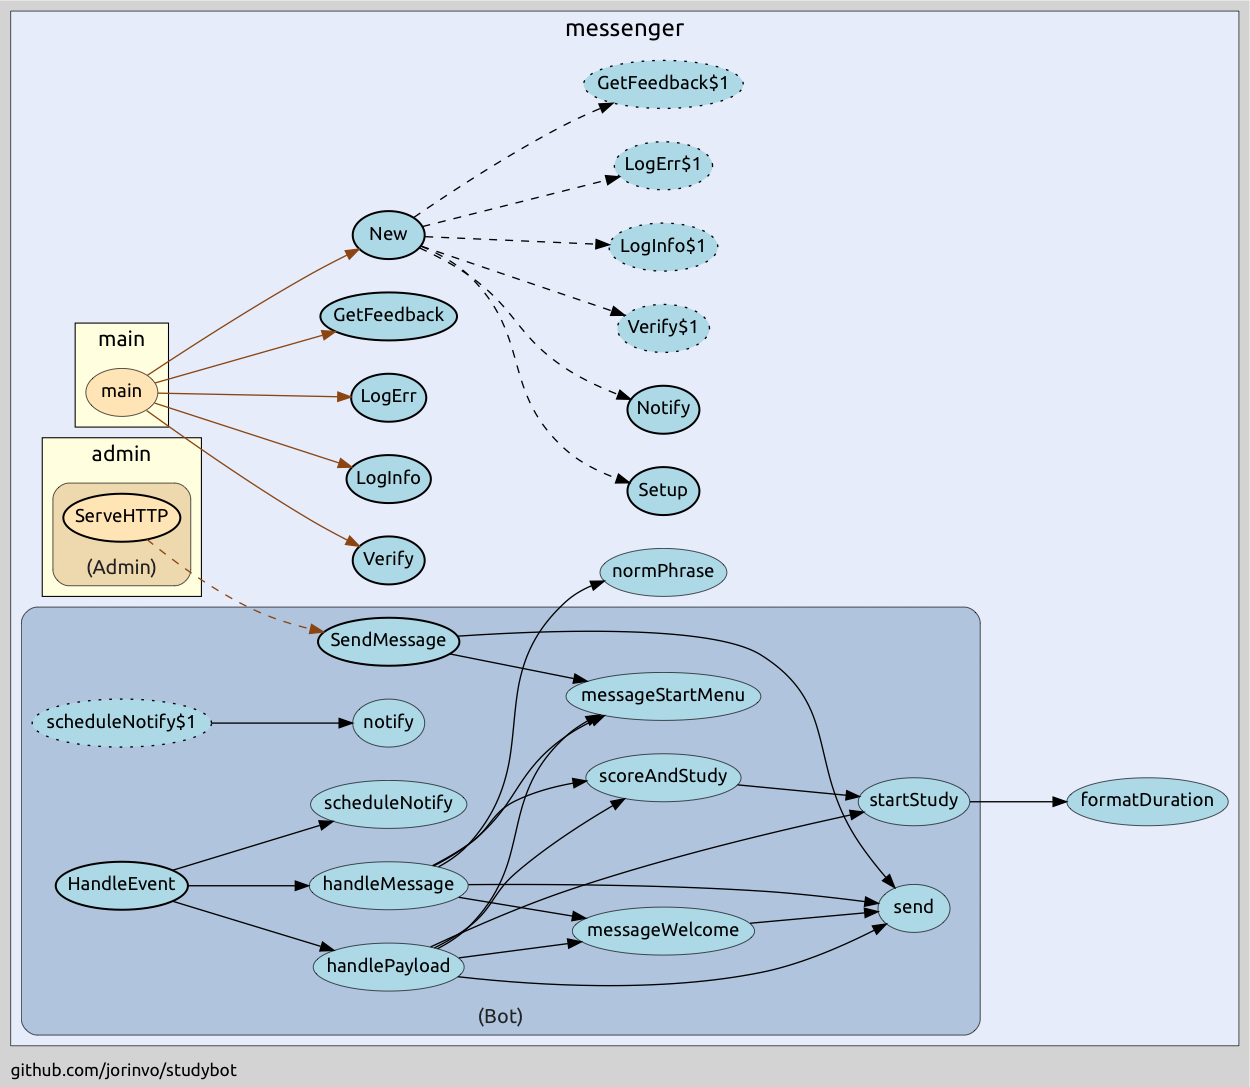
\includegraphics[width=0.8\textwidth]{images/call-graph-messenger.png}
	\caption{Call Graph of the messenger package\protect\footnotemark}
	\label{fig:call-graph-messenger}
\end{figure}
\footnotetext{The visualization has been created with \emph{go-callvis}~\cite{gocallvis}}


Most of the code base and its architecture are structure the same way most other \emph{servers} are organized;
the logic specific to the development of the chatbot is contained in the package \textbf{messenger}.
Figure \ref{fig:call-graph-messenger} illustrates the behavior of this package.
For brevity calls to the packages \textbf{brain} and \textbf{fbot} are not included in the graphic.
\\
The upper half of the graphic in \ref{fig:call-graph-messenger} shows function calls,
that are invoked from package \textbf{main} for initializing an instance of the type \emph{Bot}.
\\
The type \emph{Bot} provides functionality to handle events coming from the \emph{Facebook Messenger platform}
and to send generated responses back to users.
\\
The function \emph{HandleEvent}, which can be seen in figure \ref{fig:call-graph-messenger},
is called by package \textbf{fbot} with every event the WebHook receives,
and it is the main entry-point to the chatbot logic.
By handling different types of events,
\emph{HandleEvent} tracks whenever a user reads a message,
and it sends a message back to users,
whereby it needs to be differentiated between handling text messages
and predefined buttons.
\\
In addition to directly responding to users,
\emph{HandleEvent} is also the trigger for scheduling notifications.
With every action of users, the next time they receive a notification needs to be rescheduled,
which happens in the call to the internal function \emph{scheduleNotify}.
The function in \ref{fig:call-graph-messenger} labeled as \emph{scheduleNotify\$1} is an \emph{anonymous callback function},
one for each user, that is called by the scheduled timer to send a message to a user.
\\
Further, it is visible in \ref{fig:call-graph-messenger},
that package \textbf{admin} can call a function named \emph{SendMessage} which belongs to the \emph{Bot} type.
This is used to send replies from \emph{Slack} back to users.
\\

Call graphs for the packages \textbf{main}, \textbf{admin} and \textbf{fbot} can be found in the appendix starting on page \pageref{a:call-graph}.
Additionally the Go documentation for all exported types and functions can be found on page \pageref{a:docs}.
It explains specific implementations in more detail.
\\

Separating and containing logic specific to the chosen platform, in this case \emph{Facebook Messenger},
simplifies adopting the chatbot to new platforms in the future.
\\
The development of a chatbot can be summarized as being a slight variation of already known server-side development.
Chatbot software is fundamentally a server accepting \emph{HTTP requests} from a messenger platforms and sending \emph{HTTP responses} back to the messenger platform.
Developing such a system should be familiar for developers who have created web applications with server-side rendering in the past,
since state management and request processing work in the same manner.
While the receiving of user events can be approached with known patterns, the sending of replies back to users requires a paradigm shift in thinking.
Technically, responses are also rendered and sent to users,
but the rendering has no custom underlying interface as it is the case when rendering \emph{HTML} for web pages.
Instead, primarily plain text and only few platform-specific interface elements are available for presenting content.
\\
Apart from potential use of complex natural language technology,
the main difficulty of chatbot development is the design of user interfaces for the medium \emph{chat}.
